\documentclass[12pt,a4paper]{report}

% ── Codificação e idioma ──────────────────────────────────────────────────────
\usepackage[brazil]{babel}
\usepackage[T1]{fontenc}
\usepackage[utf8]{inputenc}

% ── Margens (padrão ABNT aproximado) ─────────────────────────────────────────
\usepackage[top=3cm,bottom=2cm,left=3cm,right=2cm]{geometry}

% ── Matemática ────────────────────────────────────────────────────────────────
\usepackage{amsmath,amssymb}

% ── Tabelas ───────────────────────────────────────────────────────────────────
\usepackage{booktabs,longtable,array,multirow}

% ── Tipografia ────────────────────────────────────────────────────────────────
\usepackage{setspace}
\usepackage{indentfirst}
\usepackage{microtype}

% ── Figuras ───────────────────────────────────────────────────────────────────
\usepackage{graphicx}
\usepackage{float}

% ── Formato de capítulo: "1  Título" (sem a palavra "Capítulo") ───────────────
\usepackage{titlesec}
\titleformat{\chapter}[block]
  {\normalfont\Large\bfseries}{\thechapter}{1em}{}
\titlespacing*{\chapter}{0pt}{2ex}{1.5ex}

% ── Hyperlinks ────────────────────────────────────────────────────────────────
\usepackage[hidelinks]{hyperref}
\usepackage{xurl}

% ── Bibliogr. (autor-data) ────────────────────────────────────────────────────
\usepackage[round,authoryear]{natbib}

\onehalfspacing
\setlength{\parindent}{1.25cm}

% ─────────────────────────────────────────────────────────────────────────────
\begin{document}

% ============================================================================
% CAPA
% ============================================================================
\begin{titlepage}
  \centering
  \vspace*{1cm}
  {\large UNIVERSIDADE FEDERAL DE MINAS GERAIS}\\[0.3cm]
  {\large Instituto de Ciências Exatas}\\[0.3cm]
  {\large Estatística}\\[4cm]
  {\large Rafael Arocho}\\[4cm]
  {\Large \textbf{Efeitos de redução de dimensionalidade sobre algoritmos
      de clusterização: uma replicação sistemática}}\\[0cm]
  \vfill
  {\large Belo Horizonte}\\[0.2cm]
  {\large 2026}
\end{titlepage}

% ============================================================================
% FOLHA DE ROSTO
% ============================================================================
\begin{titlepage}
  \centering
  \vspace*{1cm}
  {\large Rafael Arocho}\\[4cm]
  {\Large \textbf{Efeitos de redução de dimensionalidade sobre algoritmos
      de clusterização: uma replicação sistemática}}\\[3cm]
  \begin{flushright}
    \begin{minipage}{0.55\textwidth}
      Monografia apresentada ao Departamento de Estatística da
      Universidade Federal de Minas Gerais, como parte dos requisitos
      necessários para a obtenção do título de bacharel em Estatística.

      \vspace{0.8cm}
      Orientador: [Nome do Orientador]
    \end{minipage}
  \end{flushright}
  \vfill
  {\large Belo Horizonte}\\[0.2cm]
  {\large 2026}
\end{titlepage}

% ============================================================================
% PÁGINAS PRÉ-TEXTUAIS (numeração romana)
% ============================================================================
\pagenumbering{roman}
\setcounter{page}{2}

% ── Agradecimentos ────────────────────────────────────────────────────────────
\chapter*{Agradecimentos}
\addcontentsline{toc}{chapter}{Agradecimentos}

[Texto de agradecimentos]

\newpage

% ── Sumário ───────────────────────────────────────────────────────────────────
\tableofcontents
\newpage

% ============================================================================
% CONTEÚDO (numeração arábica)
% ============================================================================
\pagenumbering{arabic}
\setcounter{page}{1}

% ============================================================================
\chapter{Motivação: A Maldição da Dimensionalidade}
% ============================================================================

O avanço de pesquisas e trabalhos que utilizam dados com grande
dimensionalidade, possibilitado pela facilidade da obtenção e armazenamento
desses dados, como em genética e comportamentos sociais, trouxe uma
necessidade de simplificar o processo, compreender as variáveis que trazem
informação ao estudo e agrupar casos similares para tornar a explicação mais
clara.

O estudo de métodos de redução de dimensionalidade junto com técnicas de
clusterização se tornou essencial, mas a literatura tem algumas lacunas de
trabalhos abordando os efeitos da utilização conjunta dessas técnicas. É
nesse sentido que desejamos investigar essas lacunas e testar algoritmos em
conjunto para avaliar seus desempenhos.

% ─────────────────────────────────────────────────────────────────────────────
\section{O Fenômeno}
% ─────────────────────────────────────────────────────────────────────────────

Em espaços de alta dimensão, a geometria quebra de formas contraintuitivas.
A intuição construída em 2D ou 3D falha completamente --- e os algoritmos de
clustering, que dependem de noções de \textit{proximidade} e
\textit{distância}, são as primeiras vítimas.

\begin{quote}
  \textit{``Data points become nearly equidistant and classical notions of
    similarity lose discriminative power''} \citep{amate2026}.
\end{quote}

O problema manifesta-se de quatro formas principais em espaços de alta
dimensão:

\begin{itemize}
  \item Distâncias euclidianas entre pares de pontos convergem para o mesmo
        valor;
  \item K-Means, AHC e GMM dependem de distância, fazendo com que a
        estrutura de clusters desapareça;
  \item A separação entre clusters fica indistinguível do ruído;
  \item Redução não é pré-processamento opcional, é o que restaura o sinal.
\end{itemize}

% ─────────────────────────────────────────────────────────────────────────────
\section{Concentração de Distâncias}
% ─────────────────────────────────────────────────────────────────────────────

Para $x_1, \ldots, x_n \overset{iid}{\sim} \mathcal{N}(0, I_d)$, a
distância quadrática entre dois pontos é:
%
\begin{equation}
  d_{ij}^2 = \|x_i - x_j\|_2^2 = \sum_{k=1}^{d}(x_{ik} - x_{jk})^2.
\end{equation}

Cada parcela $(x_{ik} - x_{jk})^2$ segue distribuição $\chi^2(1)$. Pela
\textbf{Lei dos Grandes Números}:
%
\begin{equation}
  \frac{d_{ij}^2}{d} \xrightarrow{\;a.s.\;} \mathbb{E}[(x_{ik} - x_{jk})^2]
  = 2, \quad d \to \infty.
\end{equation}

Portanto $d_{ij} \approx \sqrt{2d}$ para todo par de pontos. O
\textbf{coeficiente de variação} das distâncias é:
%
\begin{equation}
  \text{CV}[d_{ij}] = \frac{\text{SD}[d_{ij}]}{\mathbb{E}[d_{ij}]}
  \;\sim\; \frac{1}{\sqrt{d}} \;\xrightarrow{d \to \infty}\; 0.
\end{equation}

Todas as distâncias concentram-se em torno de $\sqrt{2d}$. Com $d = 500$, a
variação relativa é aproximadamente 3\%, de modo que pontos próximos e
distantes tornam-se igualmente ``distantes'' --- a noção de vizinhança
colapsa. A Tabela~\ref{tab:cv} compara o CV empírico com o valor teórico
$1/\sqrt{d}$.

\begin{table}[ht]
  \centering
  \caption{Coeficiente de variação das distâncias: empírico vs.\ teórico.}
  \label{tab:cv}
  \begin{tabular}{rcc}
    \toprule
    $d$ & $\text{CV}[d_{ij}]$ empírico & $1/\sqrt{d}$ teórico \\
    \midrule
      2 & 0{,}4472 & 0{,}7071 \\
     10 & 0{,}2094 & 0{,}3162 \\
     50 & 0{,}0993 & 0{,}1414 \\
    100 & 0{,}0702 & 0{,}1000 \\
    500 & 0{,}0314 & 0{,}0447 \\
    \bottomrule
  \end{tabular}
\end{table}

% ─────────────────────────────────────────────────────────────────────────────
\section{Teorema de Beyer et al.\ (1999)}
% ─────────────────────────────────────────────────────────────────────────────

Seja $D_{\max}(q)$ e $D_{\min}(q)$ as distâncias máxima e mínima de uma
consulta $q$ a $n$ pontos. Sob condições gerais sobre a distribuição dos
dados, \citet{beyer1999} mostraram que:
%
\begin{equation}
  \lim_{d \to \infty}
  \Pr\!\left[\frac{D_{\max}(q) - D_{\min}(q)}{D_{\min}(q)} < \varepsilon\right]
  = 1, \quad \forall\,\varepsilon > 0.
\end{equation}

A consequência direta é que o vizinho mais próximo torna-se tão distante
quanto qualquer outro ponto --- algoritmos como KNN, K-Means e DBSCAN perdem
a capacidade discriminativa.

% ─────────────────────────────────────────────────────────────────────────────
\section{Concentração de Volume na Hiperesfera}
% ─────────────────────────────────────────────────────────────────────────────

A fração do volume de uma bola $d$-dimensional de raio $R$ contida na casca
exterior de espessura $\delta$ é dada por:
%
\begin{equation}
  F(d,\, \delta/R) = 1 - \left(1 - \frac{\delta}{R}\right)^{\!d}.
\end{equation}

Com $\delta/R = 0{,}01$ (apenas 1\% do raio), a fração que fica fora do
núcleo é apresentada na Tabela~\ref{tab:vol}.

\begin{table}[ht]
  \centering
  \caption{Fração do volume na casca exterior ($\delta/R = 0{,}01$).}
  \label{tab:vol}
  \begin{tabular}{rc}
    \toprule
    $d$   & $F(d,\; 0{,}01)$ \\
    \midrule
       2  & 2{,}0\%    \\
      10  & 9{,}6\%    \\
      50  & 39{,}5\%   \\
     100  & 63{,}4\%   \\
     500  & 99{,}3\%   \\
    1\,000& $>$99{,}99\% \\
    \bottomrule
  \end{tabular}
\end{table}

Praticamente \textbf{todo o volume} migra para a superfície da hiperesfera.
A consequência imediata para clustering é que não existem pontos
``centrais'' --- qualquer centróide $\mu_k$ está longe de quase todos os
membros do seu cluster.

% ─────────────────────────────────────────────────────────────────────────────
\section{Impacto Direto no Clustering}
% ─────────────────────────────────────────────────────────────────────────────

A inércia total do K-Means decompõe-se em variância \textit{within} e
\textit{between} clusters:
%
\begin{equation}
  \underbrace{\sum_{i=1}^n \|x_i - \bar{x}\|^2}_{\text{Inércia total}}
  =
  \underbrace{\sum_{k=1}^K \sum_{i \in C_k} \|x_i - \mu_k\|^2}_{\text{Within-cluster } (W)}
  +
  \underbrace{\sum_{k=1}^K n_k\|\mu_k - \bar{x}\|^2}_{\text{Between-cluster } (B)}.
\end{equation}

O K-Means maximiza implicitamente a razão $B/W$. Em alta dimensão, a razão
\textbf{sinal/ruído} desta decomposição é:
%
\begin{equation}
  \text{SNR}_d = \frac{B - W}{W} \;\sim\; \frac{\Delta}{\sqrt{d}},
\end{equation}

onde $\Delta$ é a separação intrínseca dos clusters no espaço original. Com
$d = 50$ e separação $\Delta = 1$:
%
\begin{equation}
  \text{SNR}_{2} = 1{,}00 \qquad \longrightarrow \qquad
  \text{SNR}_{50} \approx \frac{1}{\sqrt{50}} \approx 0{,}14.
\end{equation}

A mesma separação que é óbvia em 2D torna-se invisível em 50D. A redução
dimensional restaura o SNR ao eliminar as dimensões que contribuem apenas
com ruído, permitindo que $B/W$ volte a discriminar os clusters.

% ============================================================================
\chapter{Réplica do Estudo de \citet{amate2026}}
% ============================================================================

% ─────────────────────────────────────────────────────────────────────────────
\section{Escopo e Desenho Experimental}
% ─────────────────────────────────────────────────────────────────────────────

O experimento replica a metodologia de \citet{amate2026} avaliando cinco
métodos de redução de dimensionalidade cruzados com quatro algoritmos de
clusterização. A Tabela~\ref{tab:dr} apresenta os métodos de redução e a
Tabela~\ref{tab:algos} os algoritmos de clusterização utilizados.

\begin{table}[ht]
  \centering
  \caption{Métodos de redução de dimensionalidade avaliados.}
  \label{tab:dr}
  \begin{tabular}{ll}
    \toprule
    Família  & Método           \\
    \midrule
    Linear   & PCA              \\
    Kernel   & Kernel PCA (RBF) \\
    Manifold & Isomap, MDS, UMAP\\
    \bottomrule
  \end{tabular}
\end{table}

\begin{table}[ht]
  \centering
  \caption{Algoritmos de clusterização avaliados.}
  \label{tab:algos}
  \begin{tabular}{ll}
    \toprule
    Algoritmo & Tipo                \\
    \midrule
    K-Means   & Centróide           \\
    AHC       & Hierárquico (Ward)  \\
    GMM       & Probabilístico (EM) \\
    OPTICS    & Baseado em densidade\\
    \bottomrule
  \end{tabular}
\end{table}

% ─────────────────────────────────────────────────────────────────────────────
\section{Pipeline Experimental}
% ─────────────────────────────────────────────────────────────────────────────

O pipeline consiste em normalização dos dados por $z$-score, aplicação
opcional de redução de dimensionalidade e, em seguida, clusterização. A
avaliação é feita pelo ARI em relação ao \textit{ground truth}. A
Tabela~\ref{tab:niveis} descreve os níveis de redução testados.

\begin{table}[ht]
  \centering
  \caption{Níveis de redução testados (para $d = 50$).}
  \label{tab:niveis}
  \begin{tabular}{lcc}
    \toprule
    Nível        & Dimensões ($d=50$) & Racional \\
    \midrule
    $k - 1$      & 1  & Limite teórico de \citet{ding2004}: \textit{subspace bound} para K-Means \\
    25\% de $d$  & 12 & Literatura de clustering textual \\
    50\% de $d$  & 25 & Prática comum com PCA aplicado \\
    \bottomrule
  \end{tabular}
\end{table}

% ─────────────────────────────────────────────────────────────────────────────
\section{Métrica de Avaliação: ARI}
% ─────────────────────────────────────────────────────────────────────────────

O \textbf{Adjusted Rand Index} \citep[ARI;][]{hubert1985} mede a
concordância entre a partição obtida e o \textit{ground truth}, corrigida
pelo acaso:
%
\begin{equation}
  \text{ARI} = \frac{\text{RI} - \mathbb{E}[\text{RI}]}
                    {\max(\text{RI}) - \mathbb{E}[\text{RI}]}
  \in [-1,\; 1],
\end{equation}

onde o Rand Index base é:
%
\begin{equation}
  \text{RI} = \frac{a + b}{\binom{n}{2}},
\end{equation}

com $a$ = número de pares no mesmo cluster em ambas as partições e $b$ =
número de pares em clusters diferentes em ambas as partições. O ARI assume
valor 1 para partição perfeita, aproximadamente 0 para resultado aleatório e
valores negativos para resultados piores que o acaso. Entre suas vantagens
estão a correção para o número de clusters $K$ e a simetria:
$\text{ARI}(U, V) = \text{ARI}(V, U)$.

% ============================================================================
\chapter{Experimento Sistemático}
% ============================================================================

Reprodução controlada da metodologia de \citet{amate2026}: cinco métodos de
redução (PCA, Kernel PCA, Isomap, MDS, UMAP) $\times$ quatro algoritmos de
clusterização (K-Means, AHC, GMM, OPTICS) $\times$ três níveis de redução
($k-1$, 25\%, 50\%) sobre quatro tipos de \textit{datasets} sintéticos em
50 dimensões.

% ─────────────────────────────────────────────────────────────────────────────
\section{Geração dos Datasets}
% ─────────────────────────────────────────────────────────────────────────────

Quatro tipos de dados sintéticos foram embebidos em 50 dimensões via
projeção gaussiana aleatória, replicando as famílias do artigo original:

\begin{itemize}
  \item \textbf{Moons} ($n = 400$, $d = 50$, $k = 2$): variedade curvilínea
        em forma de duas luas.
  \item \textbf{Circles} ($n = 400$, $d = 50$, $k = 2$): dois círculos
        concêntricos de raios diferentes.
  \item \textbf{Gaussiano-3k} ($n = 240$, $d = 50$, $k = 3$): três clusters
        gaussianos esféricos.
  \item \textbf{Gaussiano-5k} ($n = 300$, $d = 50$, $k = 5$): cinco clusters
        gaussianos esféricos.
\end{itemize}

% ─────────────────────────────────────────────────────────────────────────────
\section{Execução do Grid de Experimentos}
% ─────────────────────────────────────────────────────────────────────────────

O experimento avalia todas as combinações de 16 variantes de redução (sem
redução mais 5 métodos $\times$ 3 níveis), 4 algoritmos de clusterização, 4
\textit{datasets} e 1000 repetições com sementes distintas, totalizando:
%
\begin{equation}
  16 \times 4 \times 4 \times 1000 = 256{.}000 \text{ execuções de clusterização.}
\end{equation}

% ─────────────────────────────────────────────────────────────────────────────
\section{Projeção em 2D por Método de Redução}
% ─────────────────────────────────────────────────────────────────────────────

A Figura~\ref{fig:proj2d} compara a estrutura original dos dados (sem
\textit{embedding} em alta dimensão) com as representações em duas dimensões
obtidas por cada técnica de redução. A linha ``2D original'' serve de
referência para avaliar quanto cada método recupera a estrutura verdadeira.

\begin{figure}[H]
  \centering
  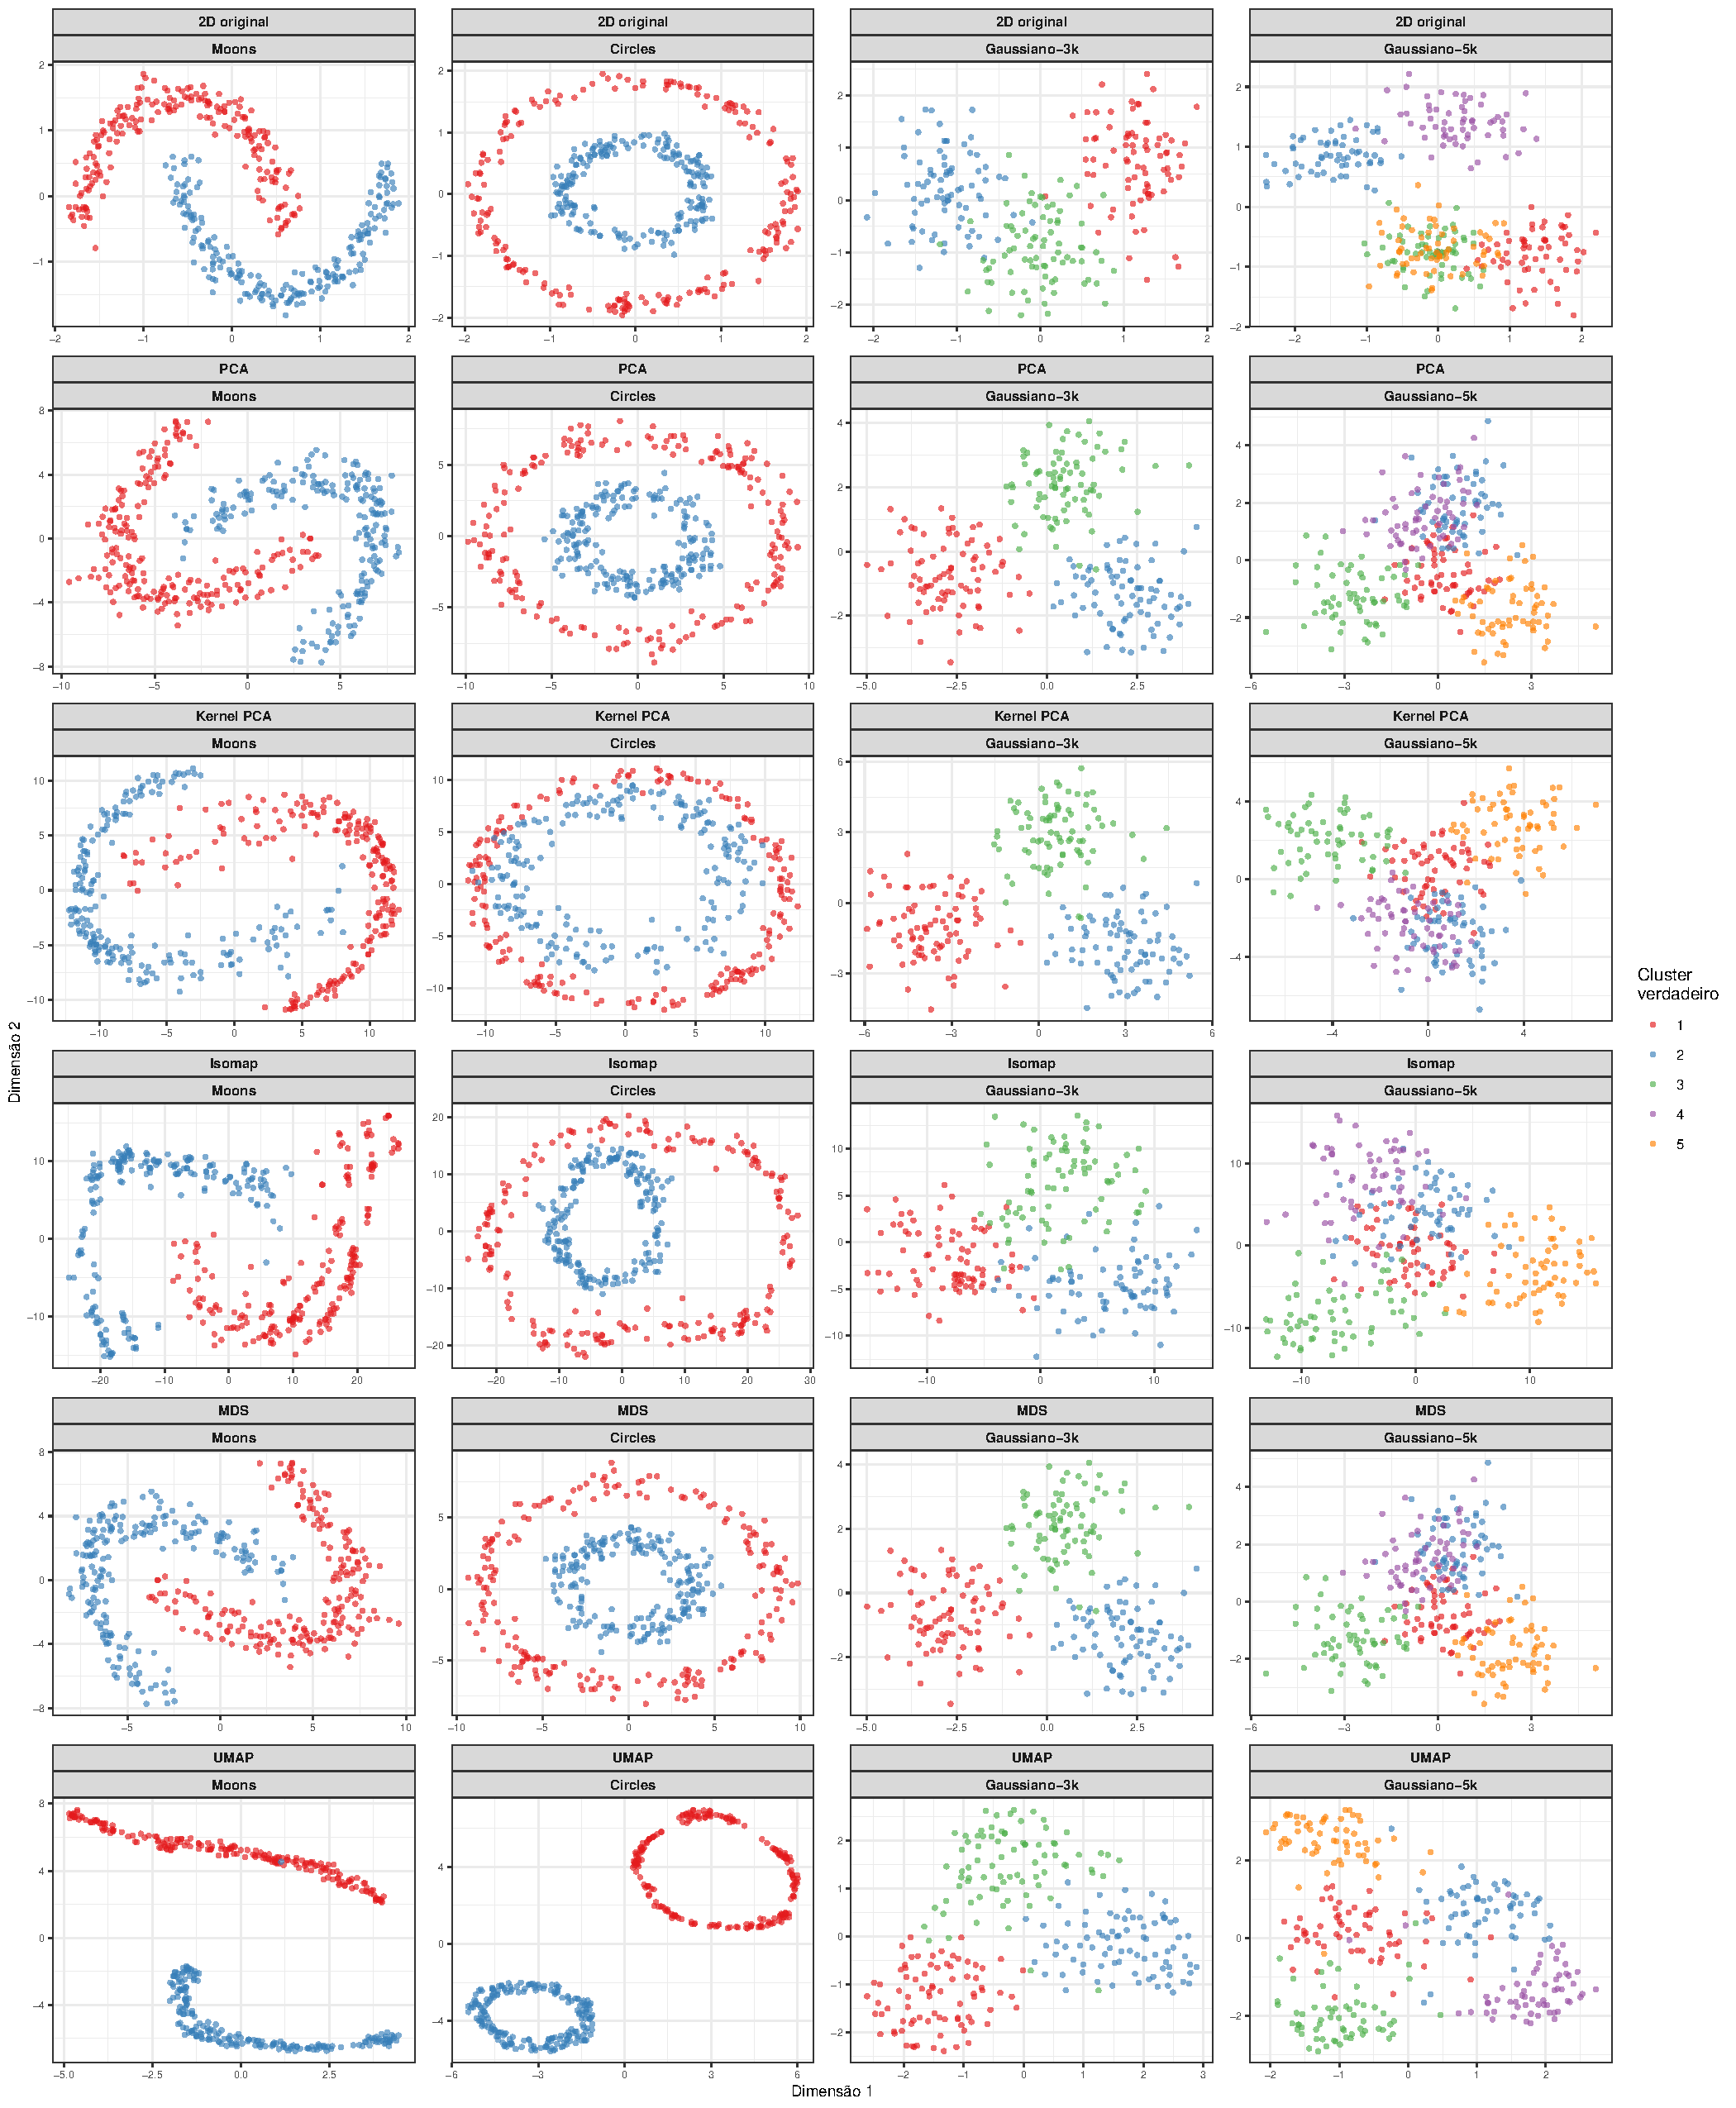
\includegraphics[width=\textwidth]{figuras/proj_2d.pdf}
  \caption{Grade 6$\times$4: linhas = método (2D original + 5 técnicas de DR),
    colunas = \textit{dataset}. A cor representa o rótulo real do cluster.}
  \label{fig:proj2d}
\end{figure}

% ─────────────────────────────────────────────────────────────────────────────
\section{Resultados: Boxplots por Algoritmo}
% ─────────────────────────────────────────────────────────────────────────────

As Figuras~\ref{fig:bp_kmeans}--\ref{fig:bp_gmm} apresentam a
distribuição do ARI (1000 réplicas) para cada combinação de método de redução
e nível, separada por \textit{dataset} e algoritmo de clusterização,
reproduzindo as Figuras~3--6 de \citet{amate2026}.

\begin{figure}[H]
  \centering
  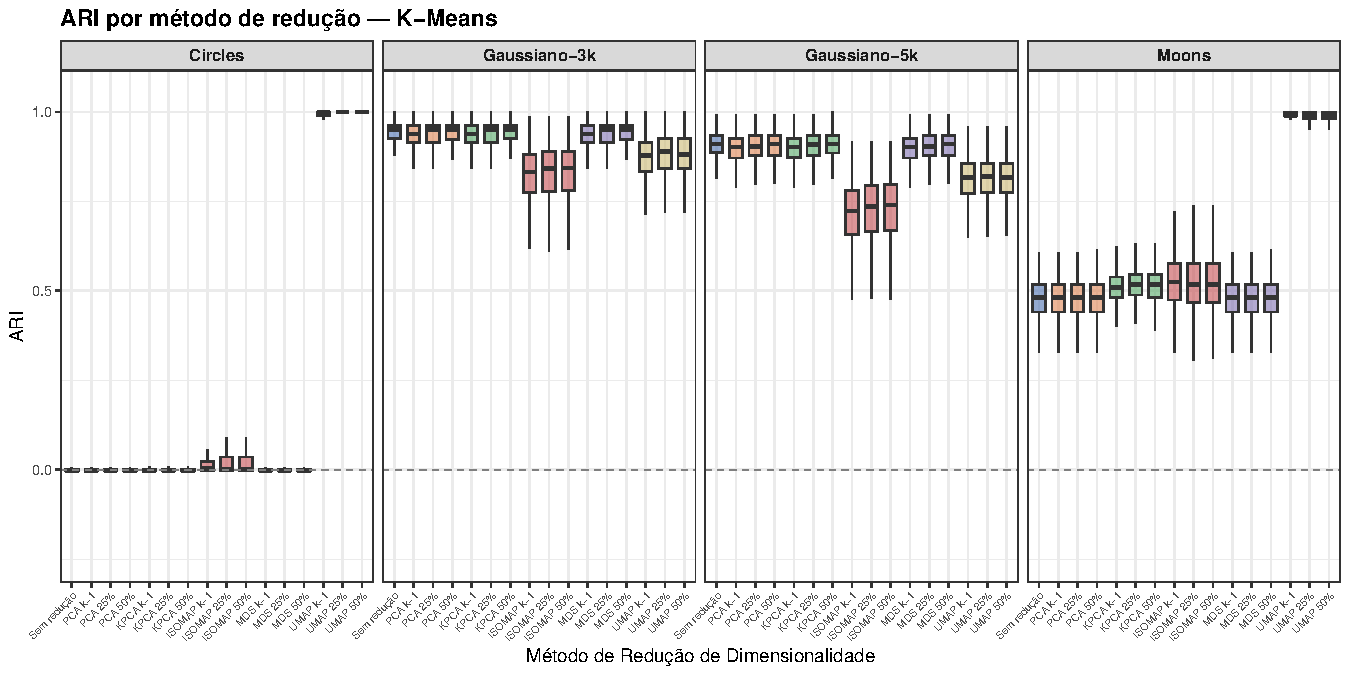
\includegraphics[width=\textwidth]{figuras/boxplot_kmeans.pdf}
  \caption{Distribuição do ARI por método de redução --- K-Means.}
  \label{fig:bp_kmeans}
\end{figure}

\begin{figure}[H]
  \centering
  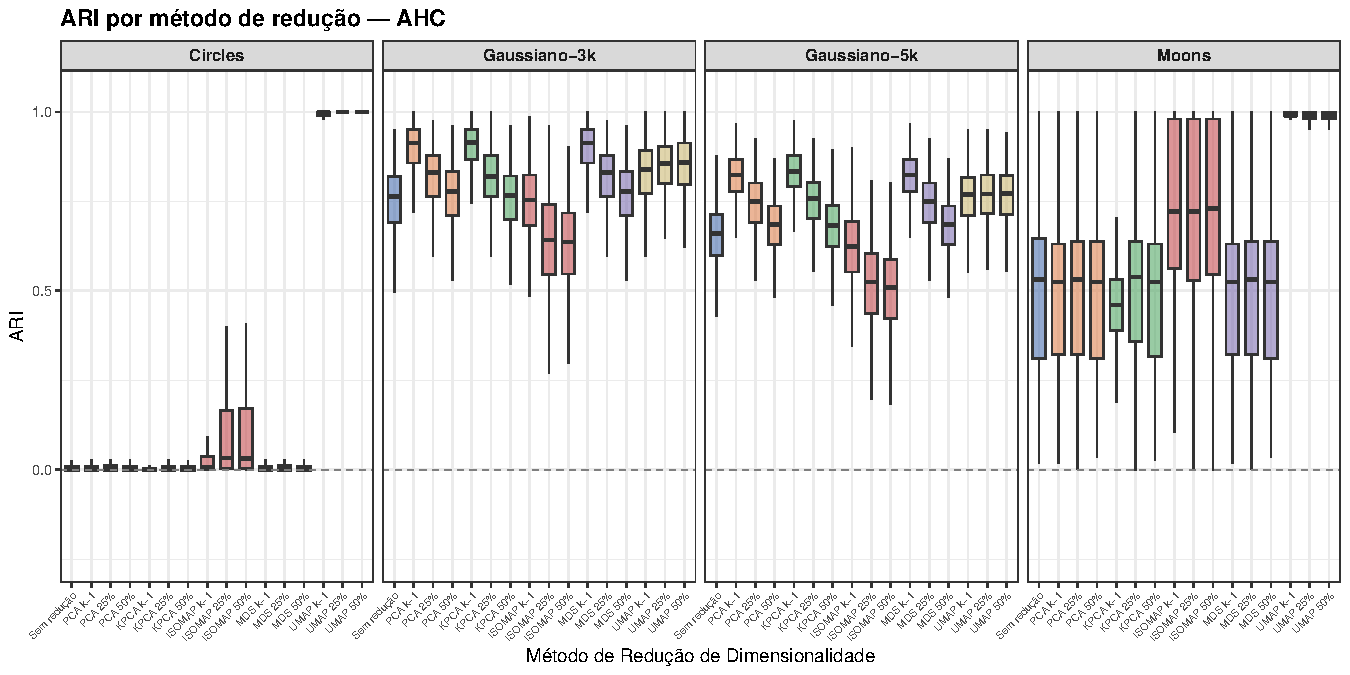
\includegraphics[width=\textwidth]{figuras/boxplot_ahc.pdf}
  \caption{Distribuição do ARI por método de redução --- AHC.}
  \label{fig:bp_ahc}
\end{figure}

\begin{figure}[H]
  \centering
  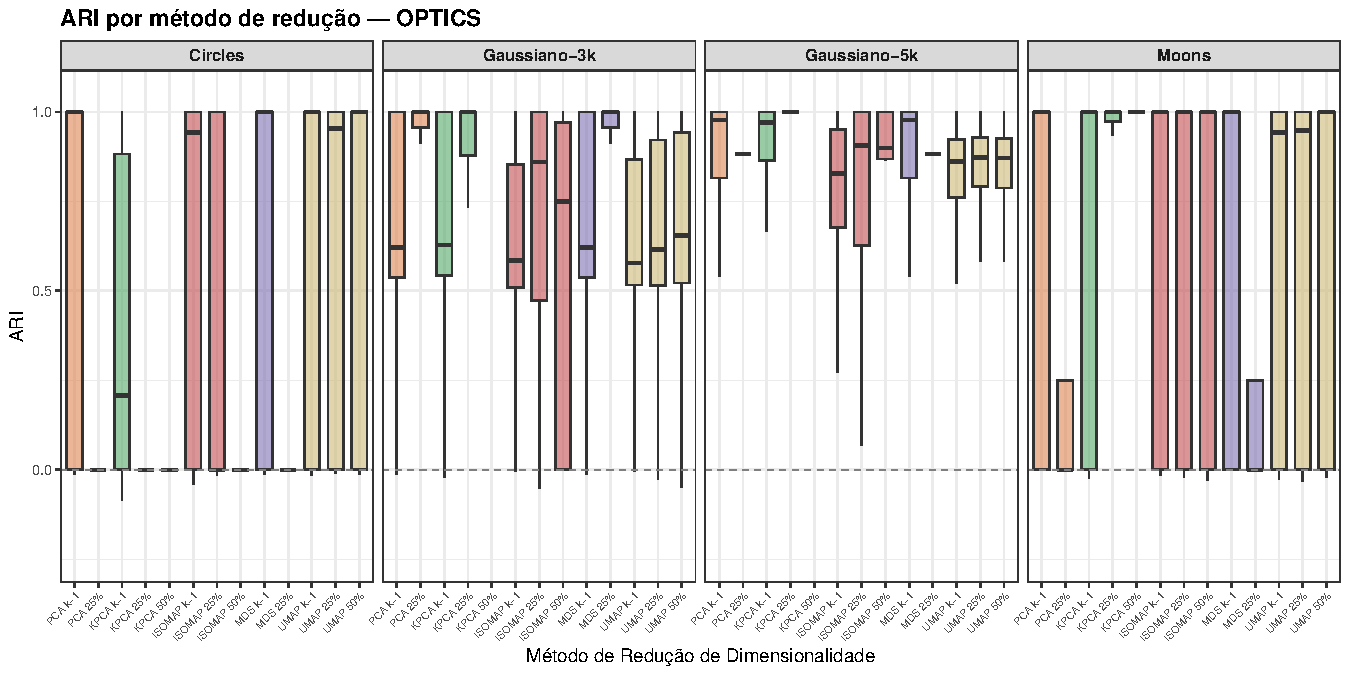
\includegraphics[width=\textwidth]{figuras/boxplot_optics.pdf}
  \caption{Distribuição do ARI por método de redução --- OPTICS.}
  \label{fig:bp_optics}
\end{figure}

\begin{figure}[H]
  \centering
  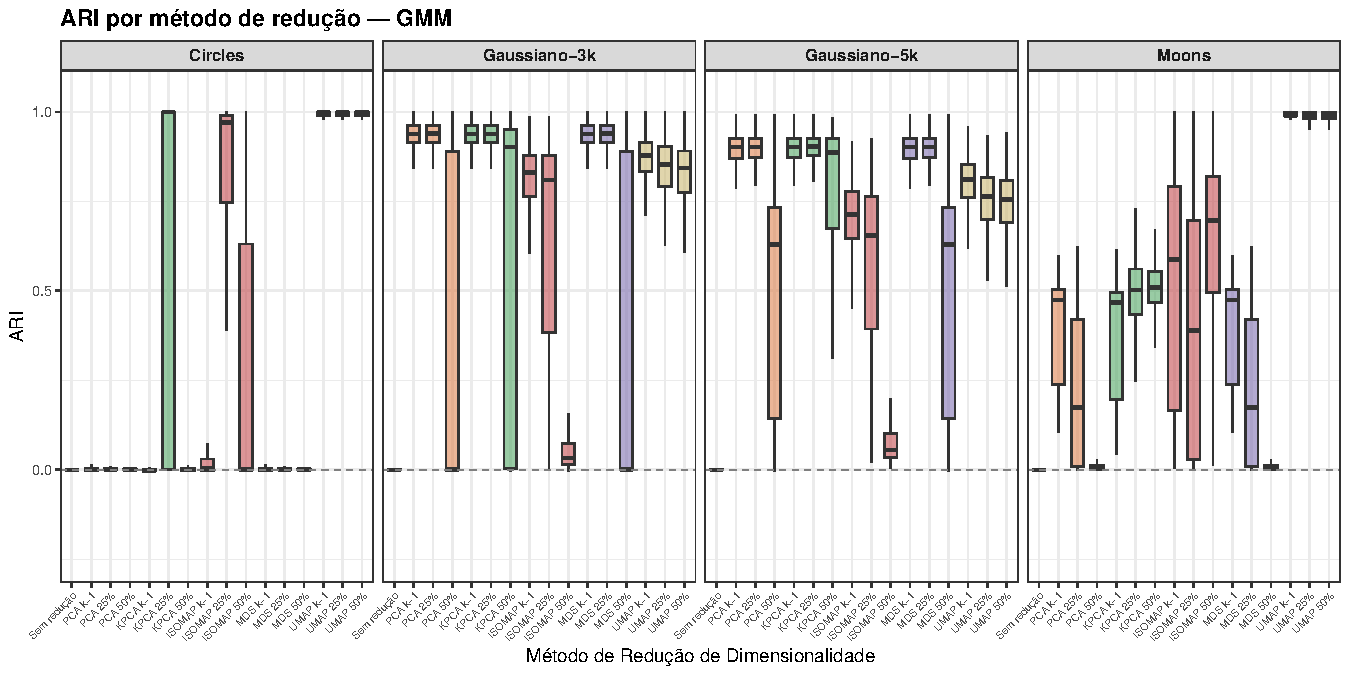
\includegraphics[width=\textwidth]{figuras/boxplot_gmm.pdf}
  \caption{Distribuição do ARI por método de redução --- GMM.}
  \label{fig:bp_gmm}
\end{figure}

% ─────────────────────────────────────────────────────────────────────────────
\section{Análise Agregada: Taxa de Vitórias}
% ─────────────────────────────────────────────────────────────────────────────

Para cada combinação DR $\times$ algoritmo, calcula-se a proporção de
casos em que a redução supera o \textit{baseline} sem redução (taxa de
vitória, WR\%) e o ganho médio de ARI ($\Delta$ARI), agregados sobre todos
os \textit{datasets}, níveis e réplicas. O OPTICS não possui
\textit{baseline} (é omitido para \texttt{sem\_reducao}), portanto sua WR
não é calculada.

\begin{table}[ht]
  \centering
  \caption{Taxa de vitória (WR\%) e ganho médio de ARI ($\Delta$ARI) por
    método de redução e algoritmo de clusterização (1000 réplicas, todos os
    \textit{datasets} e níveis). OPTICS excluído da comparação por não ter
    \textit{baseline} em alta dimensão.}
  \label{tab:winrate}
  \begin{tabular}{lcccc}
    \toprule
    \multirow{2}{*}{DR} &
      \multicolumn{4}{c}{Algoritmo} \\
    \cmidrule(lr){2-5}
    & K-Means & AHC & GMM & OPTICS \\
    \midrule
    PCA    & 15\% ($-$0{,}002) & 67\% ($+$0{,}042) &  84\% ($+$0{,}431) & --- \\
    KPCA   & 48\% ($+$0{,}007) & 64\% ($+$0{,}041) &  88\% ($+$0{,}593) & --- \\
    Isomap & 37\% ($-$0{,}050) & 47\% ($+$0{,}035) &  97\% ($+$0{,}462) & --- \\
    MDS    & 15\% ($-$0{,}002) & 67\% ($+$0{,}042) &  84\% ($+$0{,}431) & --- \\
    UMAP   & 51\% ($+$0{,}324) & 97\% ($+$0{,}411) & 100\% ($+$0{,}876) & --- \\
    \bottomrule
  \end{tabular}
\end{table}

% ─────────────────────────────────────────────────────────────────────────────
\section{Heatmap: ARI Médio por Combinação DR $\times$ Algoritmo}
% ─────────────────────────────────────────────────────────────────────────────

O \textit{heatmap} da Figura~\ref{fig:heatmap_ari} consolida o ARI médio
por método de redução (melhor nível selecionado) e algoritmo de
clusterização.

\begin{figure}[H]
  \centering
  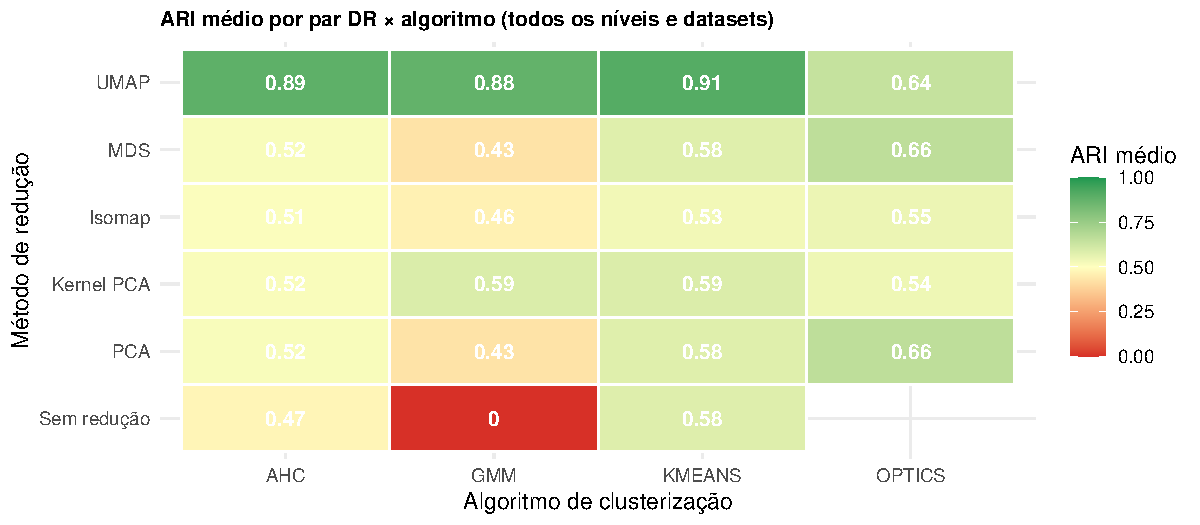
\includegraphics[width=0.85\textwidth]{figuras/heatmap_ari.pdf}
  \caption{ARI médio por par DR $\times$ algoritmo (todos os níveis e
    \textit{datasets}).}
  \label{fig:heatmap_ari}
\end{figure}

% ─────────────────────────────────────────────────────────────────────────────
\section{Efeito do Nível de Redução}
% ─────────────────────────────────────────────────────────────────────────────

A Figura~\ref{fig:niveis} investiga se o nível de compressão ($k-1$, 25\%,
50\%) impacta o ARI de forma consistente entre algoritmos e
\textit{datasets}.

\begin{figure}[H]
  \centering
  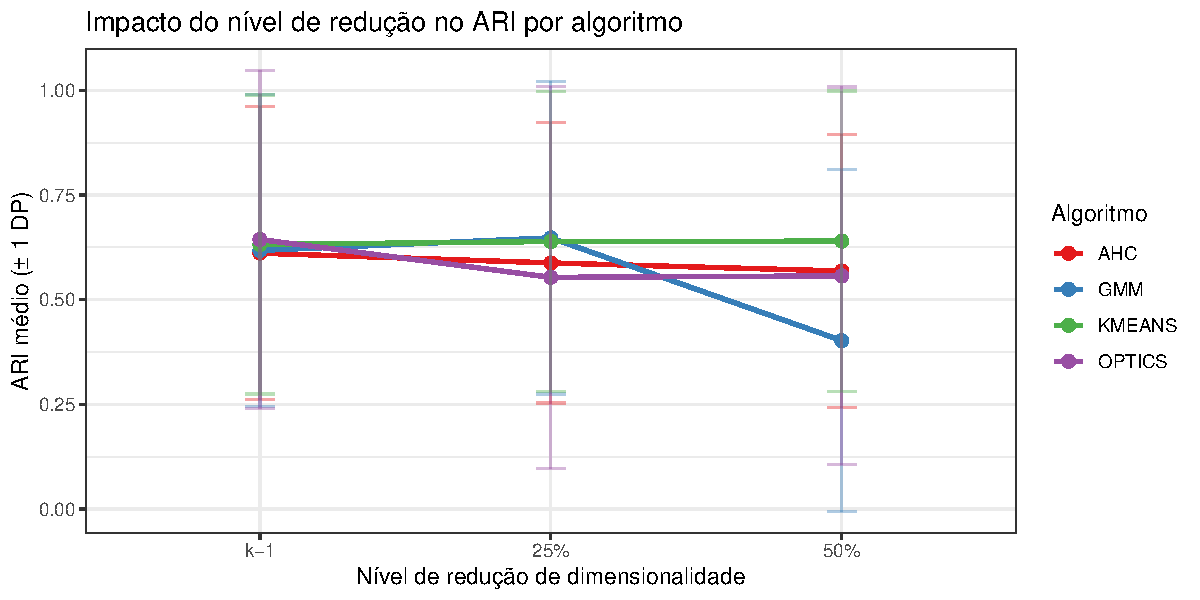
\includegraphics[width=0.80\textwidth]{figuras/niveis_reducao.pdf}
  \caption{ARI médio ($\pm 1$ DP) por nível de redução e algoritmo.}
  \label{fig:niveis}
\end{figure}

% ─────────────────────────────────────────────────────────────────────────────
\section{Custo Computacional}
% ─────────────────────────────────────────────────────────────────────────────

Cada chamada de DR e de clusterização foi cronometrada individualmente com
\texttt{proc.time()}, permitindo calcular o tempo real acumulado de cada
combinação diretamente a partir das medições. O custo atribuído a cada par
(DR, algoritmo) divide o tempo de redução entre os 4 algoritmos que
consomem a mesma projeção:
%
\begin{equation}
  \text{Custo atribuído} = \frac{t_{\text{DR}}}{4} + t_{\text{clustering}}.
\end{equation}

A Tabela~\ref{tab:tempo_dr} apresenta o tempo médio por chamada e o total
acumulado\footnote{Os tempos acumulados somam as medições individuais de
cada \textit{worker} paralelo; o tempo de parede (\textit{wall-clock}) real
é aproximadamente $\text{Total} / n_{\text{cores}}$.} para cada método de
redução. O UMAP domina amplamente o custo de DR, com média de 5\,007\,ms
por chamada e 60\,084\,s acumulados no experimento --- mais de doze vezes o
custo do Isomap.

\begin{table}[ht]
  \centering
  \caption{Tempo medido por método de redução (1000 réplicas, execução
    paralela). Cada aplicação de DR é contada uma vez (sem duplicação pelo
    número de algoritmos).}
  \label{tab:tempo_dr}
  \begin{tabular}{lrrr}
    \toprule
    Método  & Tempo médio (ms) & DP (ms) & Total acumulado (s) \\
    \midrule
    UMAP    & 5\,007 & 296\,791 & 60\,084{,}0 \\
    Isomap  &   413  &     204  &  4\,960{,}0 \\
    KPCA    &   152  &   1\,933 &  1\,820{,}0 \\
    MDS     &   102  &      53  &  1\,224{,}0 \\
    PCA     &     5  &       8  &     65{,}4  \\
    \bottomrule
  \end{tabular}
\end{table}

Do lado da clusterização, a Tabela~\ref{tab:tempo_algo} revela uma
assimetria expressiva: o GMM acumula 226\,846\,s no experimento --- cerca
de 425 vezes o tempo do AHC, representando 76\% do custo computacional
total --- em razão do alto desvio padrão (7\,667\,ms) causado por casos
de convergência lenta do algoritmo EM.

\begin{table}[ht]
  \centering
  \caption{Tempo medido por algoritmo de clusterização (1000 réplicas),
    somando todas as execuções do experimento.}
  \label{tab:tempo_algo}
  \begin{tabular}{lrrr}
    \toprule
    Algoritmo & Tempo médio (ms) & DP (ms) & Total acumulado (s) \\
    \midrule
    GMM       & 3\,558 & 7\,667 & 226\,846{,}0 \\
    OPTICS    &    25  &    12  &     846{,}0  \\
    K-Means   &    10  &    11  &     619{,}0  \\
    AHC       &     8  &    10  &     533{,}0  \\
    \bottomrule
  \end{tabular}
\end{table}

% ============================================================================
\chapter{Experimentos com Dados Reais}
% ============================================================================

Para validar as conclusões obtidas nos cenários sintéticos, estendemos a
análise para seis conjuntos de dados reais provenientes do UCI Machine
Learning Repository \citep{uci2019}.

A seleção cobre uma faixa ampla de dimensionalidades, de $d=4$ (Iris, Blood
Transfusion) até $d=90$ (Libras Movement), incluindo dois \textit{datasets}
de alta dimensão (WDBC com $d=30$ e Libras com $d=90$) que se aproximam do
regime estudado nos experimentos sintéticos. Ao contrário dos cenários
sintéticos controlados, esses conjuntos apresentam desafios reais como ruído
não gaussiano, sobreposição natural de classes e diferentes escalas de
variância.

% ─────────────────────────────────────────────────────────────────────────────
\section{Datasets Utilizados}
% ─────────────────────────────────────────────────────────────────────────────

A Tabela~\ref{tab:reais} sumariza as características dos seis
\textit{datasets} utilizados.

\begin{table}[ht]
  \centering
  \caption{Datasets reais utilizados nos experimentos.}
  \label{tab:reais}
  \begin{tabular}{lrrr}
    \toprule
    Dataset            & $n$  & $d$ & $k$ \\
    \midrule
    Iris               &  150 &   4 &   3 \\
    Blood Transfusion  &  748 &   4 &   2 \\
    Yeast              & 1484 &   8 &  10 \\
    Wine               &  178 &  13 &   3 \\
    WDBC               &  569 &  30 &   2 \\
    Libras Movement    &  360 &  90 &  15 \\
    \bottomrule
  \end{tabular}
\end{table}

Utilizamos o PCA (projeção linear) e o UMAP (projeção \textit{manifold}
não-linear) para inspecionar visualmente a separabilidade das classes antes
da clusterização.

% ─────────────────────────────────────────────────────────────────────────────
\section{Estrutura dos Dados Reais}
% ─────────────────────────────────────────────────────────────────────────────

A Figura~\ref{fig:reais_vis} apresenta as projeções em 2D (PCA e UMAP) dos
seis \textit{datasets} reais, ordenados por dimensionalidade crescente.

\begin{figure}[H]
  \centering
  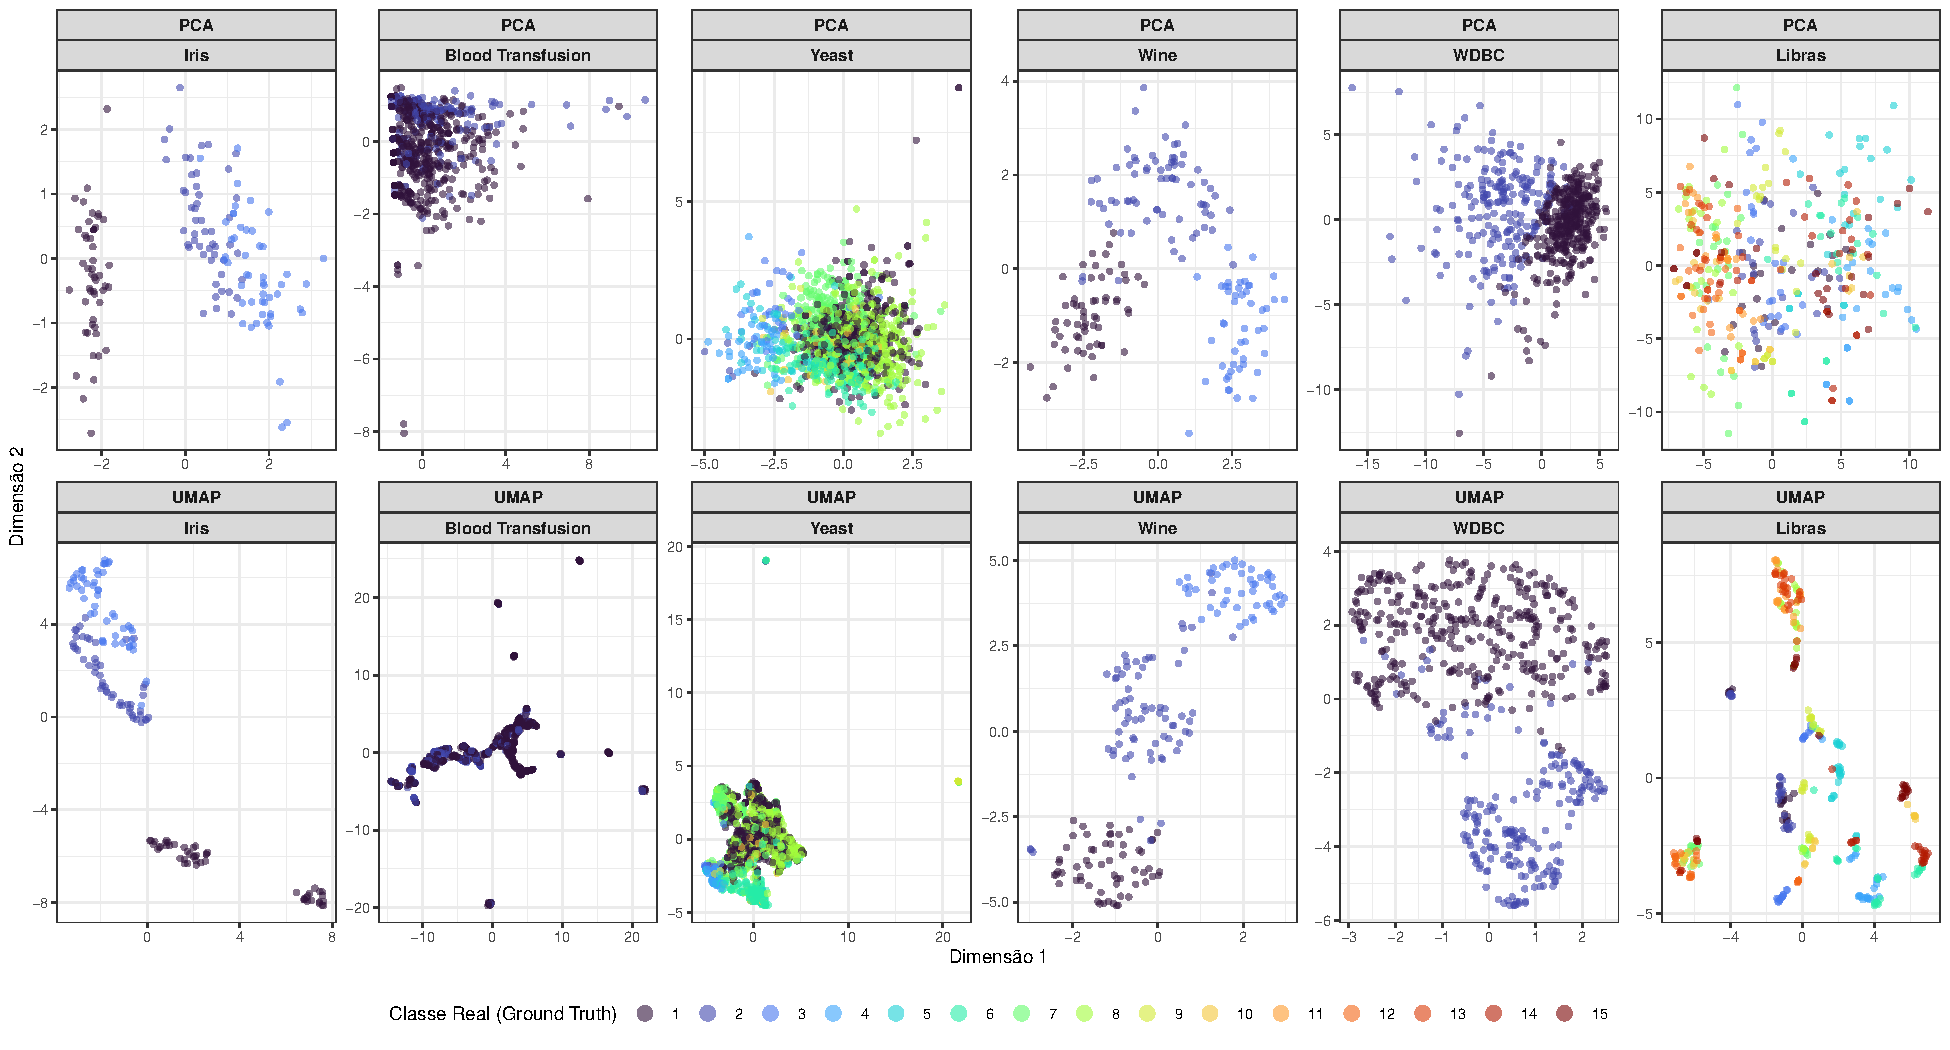
\includegraphics[width=\textwidth]{figuras/vis_reais_2d.pdf}
  \caption{Projeção em 2D dos seis \textit{datasets} reais (PCA e UMAP). A
    cor representa o rótulo real da classe.}
  \label{fig:reais_vis}
\end{figure}

% ─────────────────────────────────────────────────────────────────────────────
\section{Resultados com Dados Reais}
% ─────────────────────────────────────────────────────────────────────────────

O gráfico de lollipop da Figura~\ref{fig:heatmap_reais} apresenta o ARI por
método de redução e algoritmo, facetado por \textit{dataset}. Os
\textit{datasets} estão ordenados por dimensionalidade crescente ($d = 4$ a
$d = 90$). Células mais escuras indicam maior ARI.

\begin{figure}[H]
  \centering
  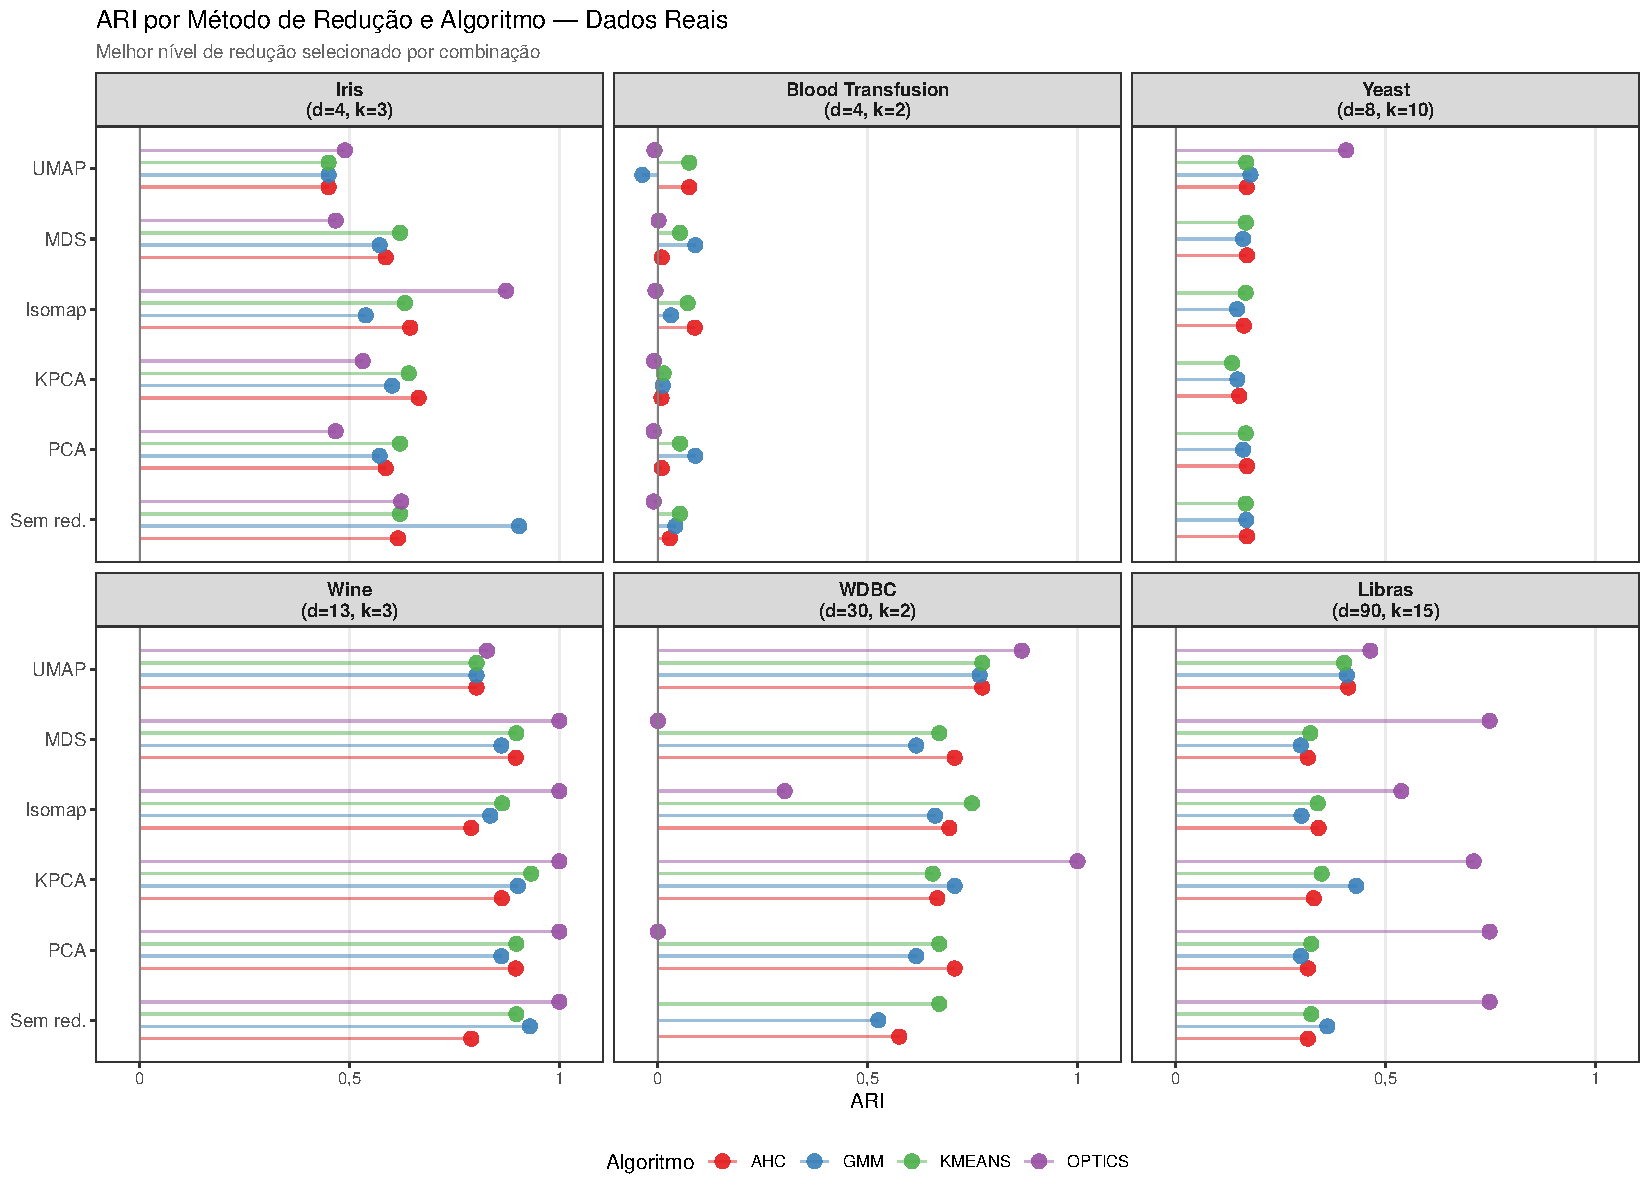
\includegraphics[width=\textwidth]{figuras/lollipop_reais.pdf}
  \caption{ARI por método de redução e algoritmo em dados reais, facetado por
    \textit{dataset} (ordenado por dimensionalidade crescente). Melhor nível
    de redução selecionado por combinação.}
  \label{fig:heatmap_reais}
\end{figure}

% ============================================================================
\chapter{Conclusões}
% ============================================================================

Os experimentos realizados --- 1000 réplicas com quatro \textit{datasets}
sintéticos em 50 dimensões e validação em seis conjuntos de dados reais ---
permitem formular conclusões precisas sobre quando e como a redução de
dimensionalidade beneficia a clusterização.

% ─────────────────────────────────────────────────────────────────────────────
\section{UMAP é o método dominante para dados manifold}
% ─────────────────────────────────────────────────────────────────────────────

O UMAP é o único método de redução que produz ganhos expressivos e
consistentes de ARI frente ao \textit{baseline} sem redução. Para o AHC,
a taxa de vitória do UMAP atinge \textbf{97\%} (com $\Delta$ARI médio de
$+0{,}41$); para o K-Means, chega a 51\% ($\Delta$ARI $\approx +0{,}32$).
Para o GMM, a taxa de vitória é de \textbf{100\%} com $\Delta$ARI médio
de $+0{,}88$ --- efeito explicado pelo colapso total do GMM sem redução
(ARI $\approx 0$, discutido na Seção~\ref{sec:gmm}).
Esse domínio é explicado pela natureza dos \textit{datasets} sintéticos: os
conjuntos Circles e Moons possuem estrutura de variedade não-linear
(\textit{manifold}), invisível por projeções lineares.

O efeito é dramático no Circles: sem redução, o ARI médio do AHC é $0{,}007$
(praticamente aleatório), pois a estrutura esférica em 50D é inteiramente
destruída pela projeção gaussiana aleatória. Com UMAP, o ARI salta para
$0{,}952$. No Moons, o ganho é de $0{,}486$ para $0{,}990$. Nenhum outro
método se aproxima dessas magnitudes.

% ─────────────────────────────────────────────────────────────────────────────
\section{A redução prejudica dados gaussianos}
% ─────────────────────────────────────────────────────────────────────────────

Para os \textit{datasets} Gaussiano-3k e Gaussiano-5k, a separabilidade
linear em 50 dimensões já é suficientemente alta para o K-Means (ARI médio
$\approx 0{,}94$ e $0{,}91$ sem redução). Nesses casos, o UMAP
\textit{prejudica} o K-Means (de $0{,}942$ para $0{,}877$ no
Gaussiano-3k; de $0{,}909$ para $0{,}812$ no Gaussiano-5k). O AHC, por
outro lado, parte de ARI menor ($0{,}75$ no Gaussiano-3k) e ainda ganha com
UMAP ($+0{,}09$). O Isomap é o método com menor ARI médio nesse cenário
($0{,}51$ para o AHC no Gaussiano-3k).

Isso confirma a hipótese teórica com uma nuance importante: a redução
beneficia ou prejudica \textit{dependendo do algoritmo}. Para o K-Means,
que já explora a separabilidade linear de 50D, a redução pode descartar
dimensões informativas. Para o AHC, menos sensível à escala global das
distâncias, mesmo uma leve compressão ainda traz ganho.

% ─────────────────────────────────────────────────────────────────────────────
\section{PCA e MDS produzem resultados equivalentes}
% ─────────────────────────────────────────────────────────────────────────────

PCA e MDS apresentam ARI médio idêntico ($0{,}523$) em todos os
\textit{datasets} e algoritmos. Isso é esperado: em dados euclidianos
normalizados, o MDS por coordenadas clássicas é algebricamente equivalente
ao PCA. A diferença prática é o custo: PCA leva em média $5$\,ms por
chamada, enquanto MDS consome $102$\,ms --- razão de aproximadamente 20:1.
Para dados euclidianos, o PCA é empiricamente preferível sem perda de
qualidade.

% ─────────────────────────────────────────────────────────────────────────────
\section{OPTICS e a maldição da dimensionalidade}
% ─────────────────────────────────────────────────────────────────────────────

O OPTICS não pôde ser avaliado no \textit{baseline} sem redução (50D): a
concentração de distâncias em alta dimensão destrói os gradientes de
densidade necessários para extrair clusters coerentes. Após redução, o
OPTICS funciona bem, e as melhores configurações são PCA e MDS com nível
$k-1$ (ARI médio $0{,}669$). O UMAP não é o melhor parceiro para o OPTICS:
a distorção topológica local do algoritmo interfere com as vizinhanças de
densidade que o OPTICS explora.

% ─────────────────────────────────────────────────────────────────────────────
\section{O GMM colapsa em alta dimensão e se recupera com UMAP}
\label{sec:gmm}
% ─────────────────────────────────────────────────────────────────────────────

O GMM é o algoritmo mais sensível à dimensionalidade entre os quatro
avaliados. Sem redução de dimensionalidade, o ARI médio do GMM é
\textbf{0{,}000} em todos os \textit{datasets} sintéticos em 50D --- o pior
resultado de todo o experimento. O algoritmo EM, ao estimar matrizes de
covariância em 50 dimensões a partir de 240--400 observações, enfrenta
condicionamento numérico extremamente ruim, fazendo com que as atribuições
de cluster sejam essencialmente aleatórias.

Com UMAP, o GMM atinge ARI médio de \textbf{0{,}876} --- taxa de vitória de
100\% sobre o \textit{baseline} e resultado comparável ao K-Means + UMAP
($0{,}906$). O KPCA também recupera o GMM de forma expressiva (ARI
$= 0{,}590$), sugerindo que a projeção em espaço de características de
kernel captura estrutura suficiente para que as gaussianas do modelo sejam
identificáveis.

O custo desse desempenho é alto: o GMM acumula 226\,846\,s de tempo de
execução --- 76\% do custo computacional total do experimento --- com
desvio padrão de 7\,667\,ms por chamada, reflexo de casos de convergência
lenta do EM. A combinação UMAP + GMM oferece qualidade próxima ao
UMAP + K-Means, porém a um custo de clusterização cerca de 356 vezes
maior.

% ─────────────────────────────────────────────────────────────────────────────
\section{O nível mais agressivo é o mais eficaz}
% ─────────────────────────────────────────────────────────────────────────────

O nível $k-1$ é o mais agressivo das três opções: para os \textit{datasets}
com $k=2$ (Moons, Circles), reduz de 50D para \textbf{1D}; para $k=3$
(Gaussiano-3k), para 2D; para $k=5$ (Gaussiano-5k), para 4D. Ainda assim,
supera consistentemente os níveis 25\% (12D) e 50\% (25D) --- ARI médio:
$0{,}626$ vs.\ $0{,}616$ e $0{,}539$.

Esse resultado, aparentemente paradoxal, tem justificativa teórica direta:
\citet{ding2004} demonstraram que a solução ótima do K-Means no espaço
completo é equivalente à solução ótima no subespaço de $k-1$ componentes
principais. Além disso, os \textit{datasets} sintéticos têm dimensão
intrínseca exatamente $k-1$: Moons e Circles são variedades 1D embebidas em
50D; os Gaussianos são separáveis em $k-1$ hiperplanos. As dimensões além
de $k-1$ são ruído gaussiano puro introduzido pela projeção aleatória.
Portanto, comprimir até $k-1$ \textit{elimina} o ruído sem perder sinal,
enquanto os níveis 25\% e 50\% retêm parte desse ruído.

% ─────────────────────────────────────────────────────────────────────────────
\section{Custo computacional e fronteira qualidade-custo}
% ─────────────────────────────────────────────────────────────────────────────

O UMAP domina o custo de redução: $5{.}007$\,ms por chamada em média e
$60{.}084$\,s acumulados no experimento, contra $5$\,ms e $65{,}4$\,s do
PCA --- razão de 1001:1. O Isomap é o segundo mais caro ($413$\,ms) e
apresenta ARI médio de $0{,}53$ para o K-Means, abaixo do desempenho do
UMAP, configurando baixo retorno em custo-benefício.

A fronteira qualidade-custo mais eficiente é ocupada pelo par
\textbf{PCA/KPCA + AHC}: ARI médio competitivo ($\approx 0{,}52$)
com custo de DR inferior a $160$\,ms por chamada. O UMAP + K-Means oferece
a melhor qualidade absoluta ($0{,}906$), mas a custo de DR mais de 1000
vezes maior que PCA + K-Means.

% ─────────────────────────────────────────────────────────────────────────────
\section{Validação com dados reais}
% ─────────────────────────────────────────────────────────────────────────────

Os experimentos com dados reais confirmam as conclusões sintéticas. Os
maiores ganhos de DR ocorrem em \textit{datasets} de alta dimensão:
\begin{itemize}
  \item \textbf{WDBC} ($d=30$, $k=2$): UMAP + AHC eleva o ARI de $0{,}575$
        para $0{,}773$ ($+0{,}198$); OPTICS + KPCA alcança ARI perfeito
        ($1{,}000$).
  \item \textbf{Libras} ($d=90$, $k=15$): UMAP + AHC ganha $+0{,}096$
        (de $0{,}314$ para $0{,}411$).
  \item \textbf{Wine} ($d=13$, $k=3$): PCA + AHC ganha $+0{,}106$
        (de $0{,}790$ para $0{,}896$).
\end{itemize}
Em \textit{datasets} de baixa dimensão (Iris com $d=4$, Blood Transfusion
com $d=4$, Yeast com $d=8$), os ganhos são modestos (máximo $\Delta < 0{,}06$,
exceto Iris com Isomap + OPTICS, $\Delta = 0{,}250$). O padrão é claro:
a DR é mais valiosa quando a dimensionalidade intrínseca dos dados é baixa
mas o espaço observado é alto.

% ─────────────────────────────────────────────────────────────────────────────
\section{Síntese}
% ─────────────────────────────────────────────────────────────────────────────

\begin{enumerate}
  \item \textbf{A redução de dimensionalidade não beneficia universalmente a
        clusterização}: o ganho depende criticamente da estrutura intrínseca
        dos dados e do algoritmo de clusterização escolhido.
  \item \textbf{UMAP é indispensável para variedades não-lineares}: é o único
        método capaz de recuperar estruturas curvilíneas destruídas pela
        maldição da dimensionalidade, com taxa de vitória de 97\% para o AHC
        ($\Delta\text{ARI} \approx +0{,}41$).
  \item \textbf{PCA domina em eficiência para dados lineares}: idêntico ao MDS
        em qualidade ($0{,}523$), aproximadamente 20 vezes mais rápido.
  \item \textbf{O nível de redução $k-1$ é o mais eficaz, apesar de ser o
        mais agressivo}: reduzir até a dimensão intrínseca ($k-1$) elimina
        ruído puro sem perder sinal discriminativo --- ao contrário dos
        níveis 25\% e 50\%, que retêm dimensões espúrias.
  \item \textbf{O GMM colapsa completamente sem redução em alta dimensão}
        (ARI $\approx 0$), mas se recupera com UMAP (ARI $= 0{,}876$). Seu
        custo é proibitivo: 76\% do tempo total do experimento.
  \item \textbf{O par recomendado para cenários de alta dimensão com estrutura
        desconhecida é UMAP + K-Means}: melhor ARI médio absoluto ($0{,}906$),
        ao custo de DR muito maior que PCA. Para cenários onde o custo
        importa, PCA + AHC oferece desempenho competitivo ($\approx 0{,}52$)
        com custo de DR mínimo.
\end{enumerate}

% ============================================================================
% REFERÊNCIAS
% ============================================================================
\bibliographystyle{plainnat}
\begin{thebibliography}{9}

\bibitem[Amate et al.(2026)]{amate2026}
Amate, Bakhtyari, Roy \& Makarenkov (2026).
\textit{Assessing the impact of dimensionality reduction on clustering
performance --- a systematic study}.
arXiv:2604.22099.

\bibitem[Beyer et al.(1999)]{beyer1999}
Beyer, Goldstein, Ramakrishnan \& Shaft (1999).
When is ``nearest neighbor'' meaningful?
\textit{Proceedings of the 7th International Conference on Database
Theory (ICDT)}, LNCS 1540, 217--235.

\bibitem[Ding \& He(2004)]{ding2004}
Ding \& He (2004).
K-means clustering via principal component analysis.
\textit{Proceedings of the 21st International Conference on Machine
Learning (ICML)}, 225--232.

\bibitem[Hubert \& Arabie(1985)]{hubert1985}
Hubert \& Arabie (1985).
Comparing partitions.
\textit{Journal of Classification}, 2(1), 193--218.

\bibitem[McInnes \& Healy(2018)]{mcinnes2018}
McInnes \& Healy (2018).
UMAP: Uniform Manifold Approximation and Projection for dimension
reduction.
\textit{arXiv:1802.03426}.

\bibitem[UCI(2019)]{uci2019}
Dua \& Graff (2019).
\textit{UCI Machine Learning Repository}.
University of California, Irvine.

\end{thebibliography}

\end{document}
